\documentclass[a4paper,12pt]{article}
% \input{../../../config.tex}
\usepackage{../../../mypackages}
\usepackage{../../../macros}


\usepackage{pgfplots}
    \pgfplotsset{
    compat=1.11,
  }

\usetikzlibrary{shapes,arrows,babel}
\tikzstyle{box}=[minimum size = 0.1cm, rectangle, draw=black, fill=gray]
% Define the global variable

% Function that meets the requirements + ways to do custom drawing
% https://tex.stackexchange.com/questions/490374/a-curve-pass-via-points-at-tikz


\def\WITH_CORRECTION{YES}


\begin{document}

\title{Fonctions - Rappels de 2nde}
\author{N. Bancel}

\sloppy  % This will apply the sloppy setting to the entire document.
\maketitle

\section{Vocabulaire des fonctions - Fonctions affines}

\begin{enumerate}
  \item A chaque nombre réel \(x\) d'un intervalle \(I\), une fonction \(f\) associe un nombre réel et un seul que l'on note \(f(x)\). Qu'est ce qu'une image ? Qu'est-ce que l'ensemble de définition ? Qu'est qu'un antécédent ? \par
  \ans{
    \begin{minipage}{0.5\textwidth}
    \begin{itemize}
      \item[$\bullet$] \(f(x)\) est \textbf{l'image} de \(x\) par la fonction \(f\)
      \item[$\bullet$] \(I\) est \textbf{l'ensemble de définition} de \(f\)
      \item[$\bullet$] Lorsque \(y = f(x)\), on dit que le nombre \(x\) est un \textbf{antécédent} du nombre \(y\) par la fonction \(f\)
    \end{itemize}
    \end{minipage}%
    \begin{minipage}{0.5\textwidth}
    \centering
    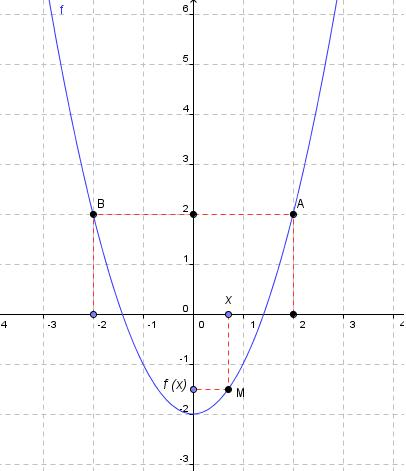
\includegraphics[width=0.5\textwidth]{image_antecedent.jpg}
    \end{minipage}
    Dans la figure ci-dessus : 
    \begin{itemize}
      \item[$\bullet$] Si M a pour abscisse \(x\), alors son ordonnée est \(f(x)\).
      \item[$\bullet$] A a pour coordonnées (2 ; 2), donc \(f(2) = 2\), donc \textbf{l’image de 2 par \(f\) est 2}.
      \item[$\bullet$] B a pour coordonnées (-2 ; 2), donc \(f(-2) = 2\) donc \textbf{l’image de -2 par \(f\) est 2}.
      \item[$\bullet$] Les \textbf{antécédents} de 2 par la fonction f sont -2 et 2.
    \end{itemize}
    }{6}{FALSE}
  \item Quelle est l'expression d'une fonction affine ? Quelle est la représentation graphique d'une fonction affine ? \par
    \ans{
      Une fonction affine est une fonction définie sur \(\mathbb{R}\) par \(f(x) = ax + b\) où  \(a\) et \(b\) désignent deux nombres réels donnés. \par
      Sa représentation graphique est une \textbf{droite} \par
      \begin{tcolorbox}
      \textbf{Vocabulaire} : Dans un repère, \(d\) est la droite représentant une fonction affine \( f : x \mapsto ax + b \)
      \begin{itemize}
        \item[$\bullet$] \textcolor{red}{a} est le \textcolor{red}{coefficient directeur} de \(d\)
        \item[$\bullet$] \textcolor{blue}{b} est \textcolor{blue}{l'ordonnée à l'origine} de \(d\) (ordonnée du point d'intersection de \(d\) avec l'axe des ordonnées)
      \end{itemize}
      \end{tcolorbox}
      \begin{minipage}{0.5\textwidth}
        \centering
        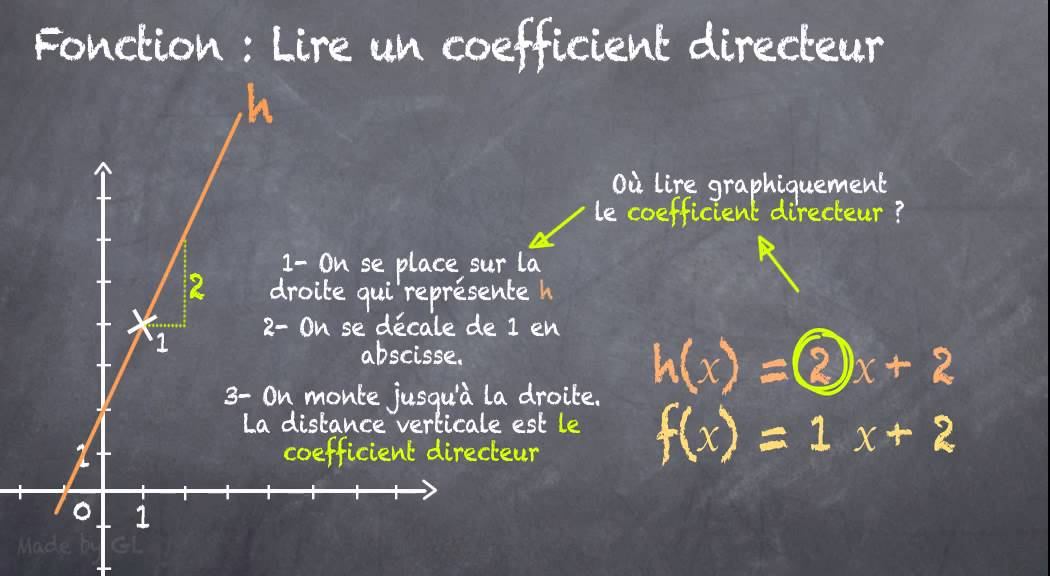
\includegraphics[width=\textwidth]{coef_directeur.jpg}
        \captionof{figure}{Source : \href{https://www.youtube.com/watch?v=ni1cSNtLgWY}{Fonction : Lire un coefficient directeur}}
      \end{minipage}
      \begin{minipage}{0.5\textwidth}
        \centering
        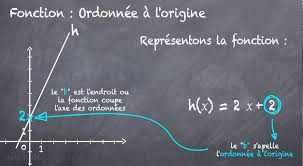
\includegraphics[width=\textwidth]{ordonnée à l'origine.jpeg}
        \captionof{figure}{Source : \href{https://www.youtube.com/watch?v=iX6LklqqPXI}{Fonction : Ordonnée à l'origine}}
      \end{minipage}
    }{4}{FALSE}
\end{enumerate}

\section{Les fonctions de référence}

\begin{enumerate}
  \item Quelle est l'expression de la fonction \textbf{carré} ? Quelle est sa propriété principale (en terme de symétrie) ? \par
  \ans{
    La fonction carré est la fonction \(f\) définie sur \(\mathbb{R}\) par \textbf{\(f(x) = x^2\)} \par 
    La représentation graphique de la fonction carré est appelée \textbf{parabole} \par
    Elle est \textbf{symétrique par rapport à l'axe des ordonées}
    \begin{figure}[H]
      \centering
      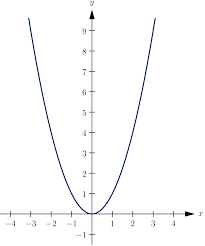
\includegraphics[width=0.3\linewidth]{carré.png}
      \caption{\label{} La fonction carré}
  \end{figure}
  }{4}{FALSE}
  \item Quelle est l'expression de la fonction \textbf{inverse} ? Quelle est sa propriété principale (en terme de symétrie) ? \par
  \ans{
    La fonction inverse est la fonction \(f\) définie sur \(\mathbb{R}\) par \textbf{\(f(x) = 1/x\)} \par 
    La représentation graphique de la fonction inverse est appelée \textbf{hyperbole} \par
    Elle est \textbf{symétrique par rapport à l'origine O du repère}
    \begin{figure}[H]
      \centering
      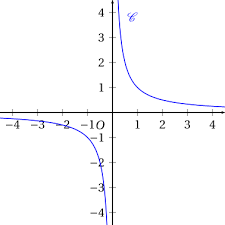
\includegraphics[width=0.3\linewidth]{inverse.png}
      \caption{\label{} La fonction inverse}
  \end{figure}
  }{4}{FALSE}
  \item Quelle est l'expression de la fonction \textbf{cube} ? Quelle est sa propriété principale (en terme de symétrie) ? \par
  \ans{
    La fonction cube est la fonction \(f\) définie sur \(\mathbb{R}\) par \textbf{\(f(x) = x^3\)} \par 
    La représentation graphique de la fonction cube est \textbf{symétrique par rapport à l'origine O du repère}
    \begin{figure}[H]
      \centering
      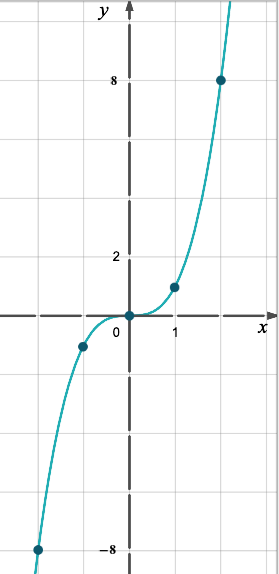
\includegraphics[width=0.25\linewidth]{cube.png}
      \caption{\label{} La fonction cube}
  \end{figure}
  }{4}{FALSE}
  \item Quelle est l'expression de la fonction \textbf{racine carrée} ? Quel est son intervalle de définition ? \par
  \ans{
    La fonction racine carrée est la fonction \(f\) définie sur l'intervalle \([0, +\infty[\). par \textbf{\(f(x) = \sqrt(x)\)} \par 
    \begin{figure}[H]
      \centering
      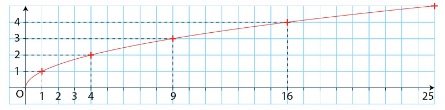
\includegraphics[width=\linewidth]{racine_carree.jpg}
      \caption{\label{} La fonction racine carrée}
  \end{figure}
  }{4}{FALSE}
\end{enumerate}

\section{Courbes représentatives des fonctions}

\begin{enumerate}
  \item A partir du graphique ci-dessous, résoudre graphiquement l'équation \(f(x) = k\) \par
  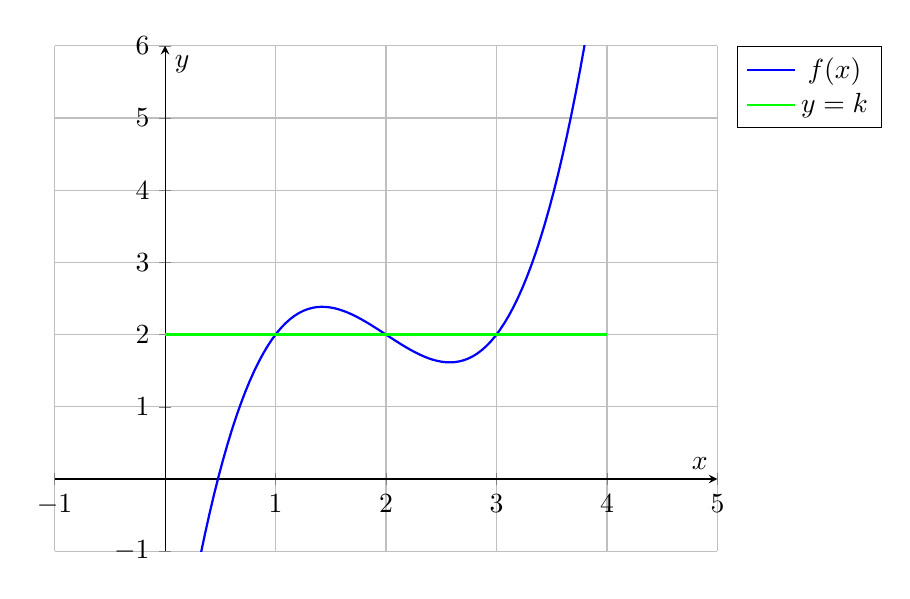
\begin{tikzpicture}
    \begin{axis}[
        axis lines = middle,
        xlabel = {$x$},
        ylabel = {$y$},
        xmin=-1, xmax=5,
        ymin=-1, ymax=6,
        domain=0:4,
        samples=100,
        legend pos=outer north east,
        grid=major,
        width=10cm, height=8cm,
    ]
    % Plot f(x) = (x-1)*(x-2)*(x-3) + 2
    \addplot[color=blue, thick] {(x-1)*(x-2)*(x-3) + 2};
    \addlegendentry{$f(x)$}
    
    % Plot y = k
    \addplot[color=green, thick] {2};
    \addlegendentry{$y = k$}
    \end{axis}
    \end{tikzpicture} \par 

  \ans{
    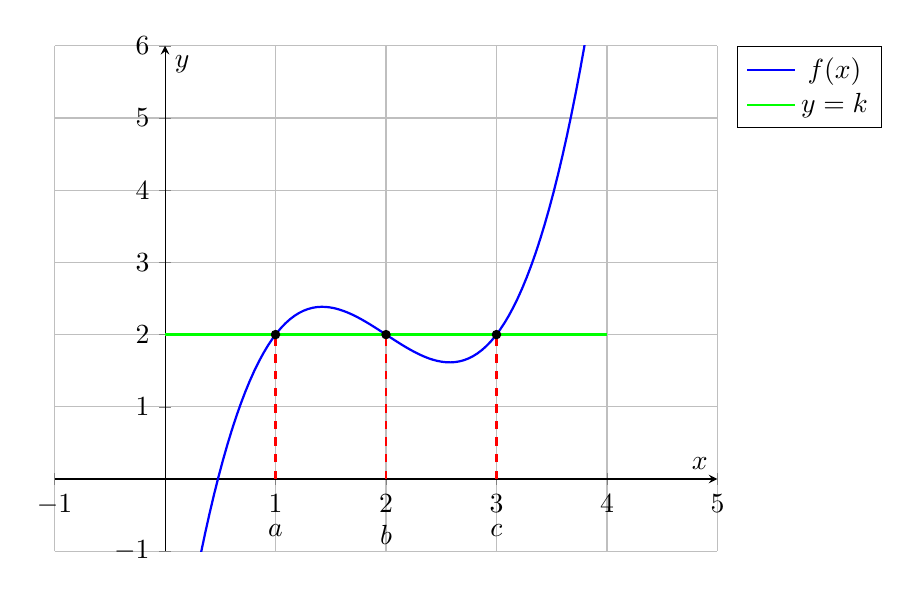
\begin{tikzpicture}
      \begin{axis}[
          axis lines = middle,
          xlabel = {$x$},
          ylabel = {$y$},
          xmin=-1, xmax=5,
          ymin=-1, ymax=6,
          domain=0:4,
          samples=100,
          legend pos=outer north east,
          grid=major,
          width=10cm, height=8cm,
      ]
      % Plot f(x) = (x-1)*(x-2)*(x-3) + 2
      \addplot[color=blue, thick] {(x-1)*(x-2)*(x-3) + 2};
      \addlegendentry{$f(x)$}
      
      % Plot y = k
      \addplot[color=green, thick] {2};
      \addlegendentry{$y = k$}
      
      % Mark the solutions
      \addplot[mark=*, mark size=1.5pt, color=black] coordinates {(1, 2)};
      \addplot[mark=*, mark size=1.5pt, color=black] coordinates {(2, 2)};
      \addplot[mark=*, mark size=1.5pt, color=black] coordinates {(3, 2)};
  
      \addplot[red, dashed, thick]
              coordinates {(1, 0) (1, 2)};
      \addplot[red, dashed, thick]
              coordinates {(2, 0) (2, 2)};
      \addplot[red, dashed, thick]
              coordinates {(3, 0) (3, 2)};
      
      % Labels for the solutions
      \node at (axis cs: 1,-0.5) [anchor=north] {$a$};
      \node at (axis cs: 2,-0.5) [anchor=north] {$b$};
      \node at (axis cs: 3,-0.5) [anchor=north] {$c$};
      
      \end{axis}
      \end{tikzpicture}
  }{6}{FALSE}
\end{enumerate}
\end{document}
